\chapter*{Introduction}
\addcontentsline{toc}{chapter}{Introduction}

% In the recent years, many researchers have been interested by the task of computer vision. 
% 	"task of computer vision" mi pripada zvlastni; task je jeden konkretni ukol, computer vision je cely velky obor, coz moc nejde dohromady; navic asi precijen zacneme trochu konkretneji
The task of reconstructing 3D information from multiple 2D photos of a real-world scene has attracted a lot of research in the last two decades and in the recent years in particular.
% 	tim padem muzeme tohle vyskrtnout 
% Particularly the problem of 3D reconstruction is being investigated a lot. 
% 	Kazdopadne pokracujme... 
% At this moment there is a great number of algorithms to solve problems in this area. 
A great number of algorithms have been proposed to solve problems in this area and several main approaches emerged. 
% Most of these approaches depend on the kind of input that is available 
% (a set of pictures -- determining is also how many pictures are taken, a video stream, etc.) 
% and also on the output that we expect.
The applicability of these approaches depends mainly on what kind of input we intend to feed the algorithm 
(an unorganized set of photos, a video stream, a pair of stereoscopic images, etc.) 
and also on what kind of output we expect the algorithm to produce (polygonal model, a disparity map). 
As a result of this progress, various real-world applications for these algorithms have appeared -- 
e.g., several camera trackers or products like Microsoft PhotoSynth. % TODO pridat referenci na web PhotoSynthu nebo na clanek

Simultaneously, both the general availability and the computational power of smartphones have improved significantly.
Mobile phones that employ the Linux-based Android software platform are currently very popular. \update{uvest procentualni podil na trhu, pridat citaci}{
The Android market share increased to almost 69\% in the year 2012 \cite{market_share}. 
See Figure \ref{fig:market_share} to compare it with the market share of the other mobile operating systems on the market in the recent two years.}
A built–in camera and a relatively fast CPUs are very common in such mobile phones.
% tahle veta by mohla jeste pokracovat ..., making it possible to...

\begin{figure}[h]
  \centering{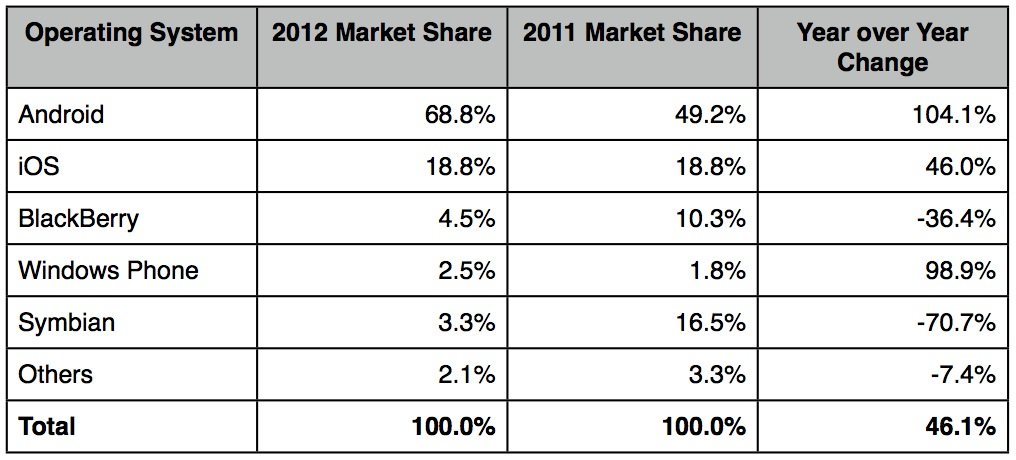
\includegraphics[width=120mm]{img/market_android_table.jpg}}
  \caption{Top five smartphone operating systems and their market share in 2011 and 2012.}
  \label{fig:market_share}
\end{figure}

The goal of this work is to explore ways how to connect these two phenomena. 
Our aim is to create an Android application that takes a set of photos using the phone's internal camera, applies a series of \cv\ algorithms to reconstruct the depth information, and visualizes the result using 3D graphics. 
Due to the inherent ambiguity of the problem, it is inevitable that our approach will be limited to particular types of scenes, for example sets of photos of highly textured surfaces. 
% TODO Tuhle vetu zatim vynechavam, protoze je moc odvazna... 
% One of our main goals is to investigate how well the solving of such a computation-intesive problem can be done within the limits of a Java-based environment running on a mobile phone or a tablet computer.

\update{nasledujici vety by se mely primo odkazovat na sekce}{}
The first part of this work analyses the problem, describes available software and gives an overview of programming libraries and languages that were used (see chapter \ref{chap:overview}). 
Secondly, we focus on the theoretical foundations of 3D reconstruction from image data (see chapter \ref{chap:notions} and \ref{chap:algorithms}). 
Then we depict the basics of android development (chapter \ref{chap:android}).
The next section is devoted to the implementation of our application.
Finally, we evaluate and benchmark the resulting application (chapter \ref{chap:implementation}).
\todo{tady bychom urcite chteli explicitneji napsat, ze vysledkem budou i nejake datasety, ale to se zvladne az to budeme mit napsane}


